\chapter{Results}\label{chap:results}
% -------------------------
%% QUOTE
\vspace*{\fill}
\epigraph{If you're doing an experiment, you should report everything that you think might make it invalid — not only what you think is right about it; other causes that could possibly explain your results; and things you thought of that you've eliminated by some other experiment, and how they worked — to make sure the other fellow can tell they have been eliminated.}%
{\textit{Surely You're Joking, Mr. Feynman!, p. 341}\\ \textsc{Richard Feynman}}
\clearpage{\thispagestyle{empty}\cleardoublepage}
%%
%% Body of the chapter
%%%%%%%%%%%%%%%%%%%%%%

In this chapter, the results from every experiment is presented in the same order as chapter \ref{chap:experimental}. 

\section{PEC nanogels}
\subsection{Gels with \ce{Cr^{3+}} as crosslinker}

Table \ref{tab:crGelsAt} shows the lowest concentration for gel formation for the different polymers used in the experiments. As seen the table, gel was only formed with Alcoflood 254 S for the highest concentration tested, namely 2 wt. \%. However, it is possible that gels could have been formed at lower concentrations in the interval between 1 wt. \% and 2 wt. \%. Alcomer 24 UK formed gel at 0.5 wt. \% but not at 0.25 wt. \%. It is possible that the highest molecular weight polymer Flopaam 5115 VHM could have formed gels at concentrations lower than 0.5 wt. \%.

\begin{table}[h]
\small
\centering
\caption{Minimum concentration for gel formation for the different polymers}
\label{tab:crGelsAt}
\begin{tabular}{c c c c >{\columncolor[gray]{0.8}}c } 
\toprule
\textbf{Name} & \textbf{Producer} & \textbf{MW} & \textbf{Concentration} & \textbf{Will gel at} \\ 
&& [MDa] & [wt\%] & [wt\%]  \\
\midrule 
Alcoflood 254 S     & BASF    & 0.5 & 0.5, 1.0 and 2.0 & 2\\
Alcomer 24 UK       & BASF    & 6 & 0.25, 0.5, 1.0 and 2.0 & $\geq 0.5$ \\ 
Flopaam 5115 VHM    & SNF Floerger    & 12+ & 0.5, 1.0 and 2.0 & $\geq 0.5$ \\ 
\bottomrule
\end{tabular}
\end{table}

In order to obtain data for testing of the simulator \--- developed for transport of nanoparticles and polymer, and with a functionality of time delayed gel formation (see Chapter \what)\--- some gel formation experiments were conducted where the polymer concentration was varied from 0.25 wt. \% to 1 wt. \% and the concentration of \ce{Cr^{3+}} was varied from 22 ppm to 113 ppm. For this series of experiments, Alcomer 24 UK was used as polymer. For concentrations higher than 22 ppm, the polymer viscosity was apparently not dependent on the cross-binder concentration (within the accuracy of the measured viscosities as discussed before). The viscosities of the solutions were measured directly after preparation and after one day of aging. Figure \ref{cht:viscAlco} shows viscosity as function of shear rate for three polymer concentrations. 
\begin{figure}
    \centering
    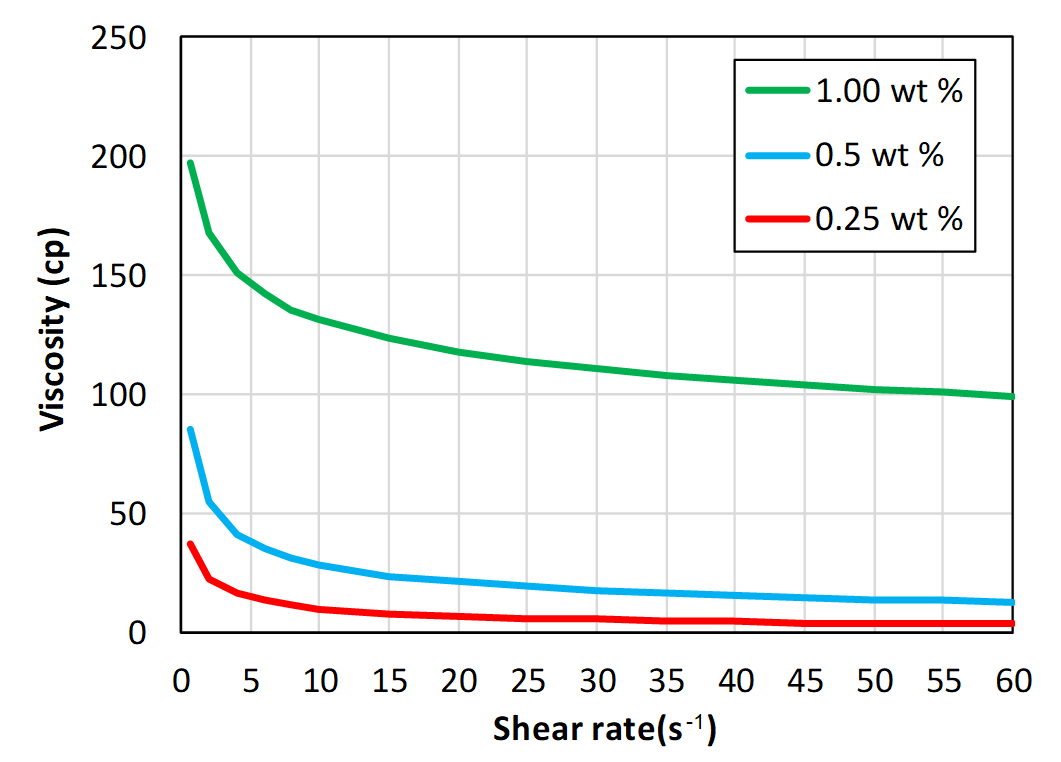
\includegraphics[width=.75\textwidth]{img/cht/viscAlcomer.png}
    \caption{Viscosity as function of shear rate and polymer concentration for Alcomer 24 UK}
    \label{cht:viscAlco}
\end{figure}

\subsection{Polyelectrolyte complexes according to the Texas A\&M recipe}

Figure \ref{cht:s10visc50} shows viscosity as function of time on logarithmic and linear scales. As shown in the figure, there were only minor increases in viscosity the first 7 days. After 23 days, the viscosity was increased significantly and it increased further when the last sample was measured after 37 days. Simple power functions were fitted to the experimental data. The plot on linear scale suggest that the largest effect of the cross binding occurred after approximately 20 days. 

\begin{figure}
    \centering
    \makebox[\textwidth][c]{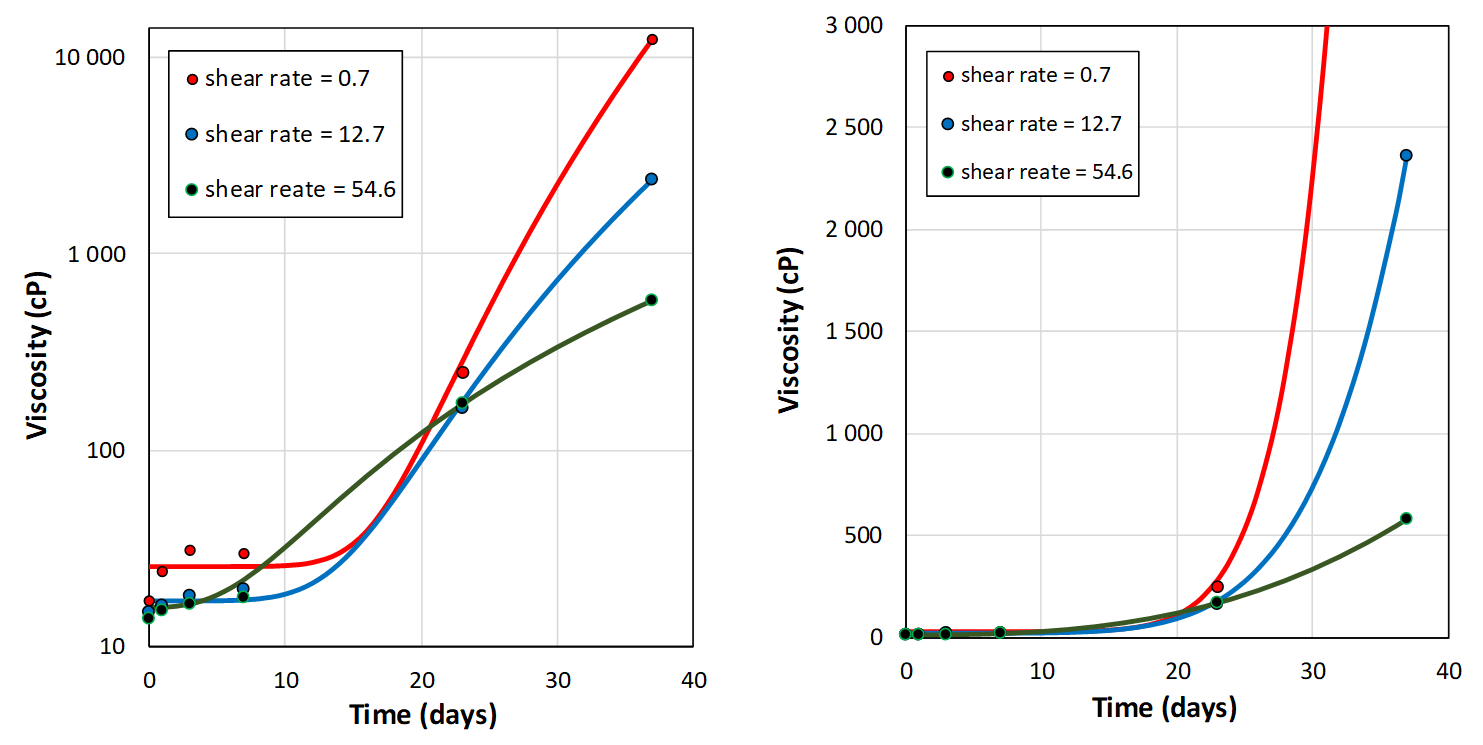
\includegraphics[width=1.2\textwidth]{img/cht/s10visc50.png}}
    \caption{Viscosity as function of aging time for Series 10 samples aged at 50~\celsius~ on logarithmic (left) and linear (right) scales}
    \label{cht:s10visc50}
\end{figure}

Figure \ref{cht:s3536visc} shows the results from viscosity measurements on Series 35 (polymer/PEC solutions made using 0.498 wt. \% of Alcomer 24 UK) and Series 36  0.490 wt. \% of Flopaam 5115 VHM). As seen in Figure \ref{cht:s3536visc}, the viscosity increased quickly, and gels were formed in the vials (visual observations) already after 3 days of aging. The apparent decrease in viscosity at longer aging times are artifacts due to the measurement method as the solutions still appeared as gels.

\begin{figure}
    \centering
    \makebox[\textwidth][c]{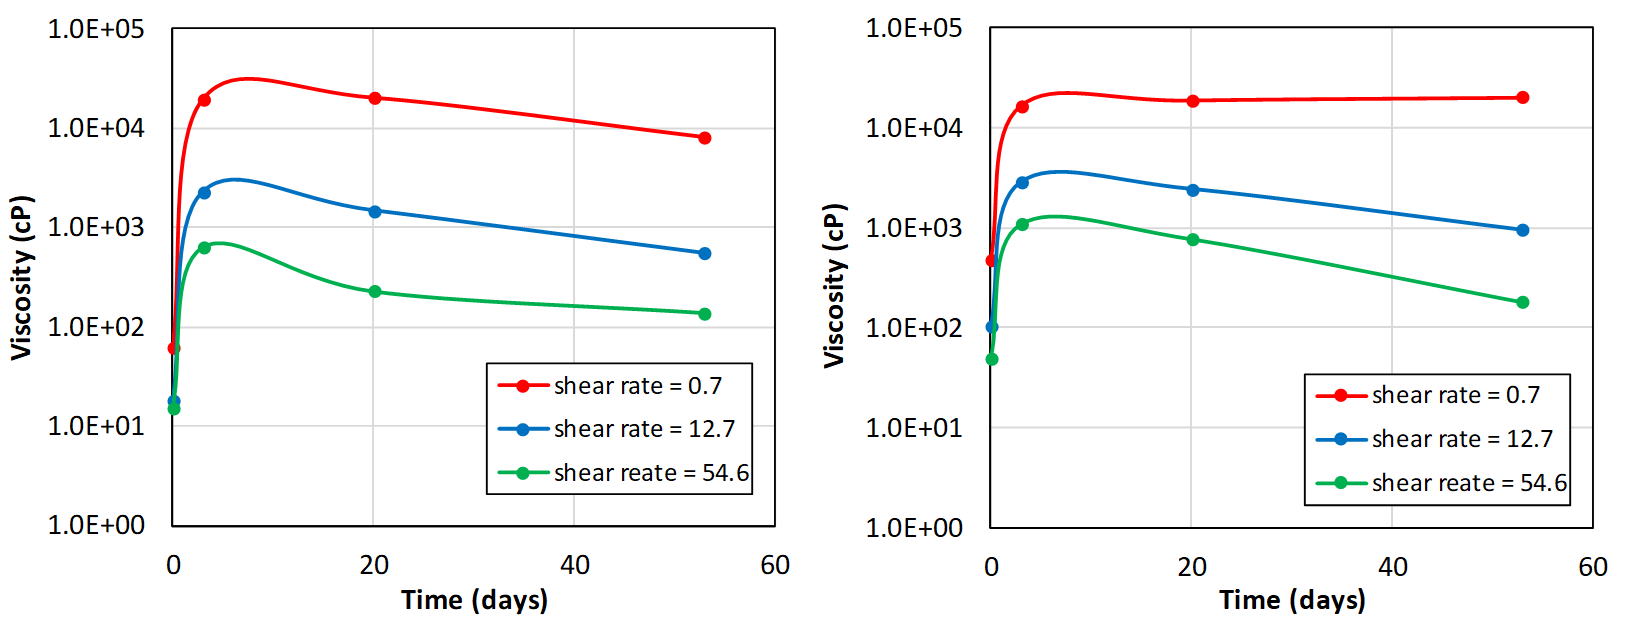
\includegraphics[width=1.2\textwidth]{img/cht/s3536.png}}%
    \caption{Viscosity as function of aging time for Series 35 samples (left) and Series 36 samples (right), aged at 80~\celsius}
    \label{cht:s3536visc}
\end{figure}

Two more systems were made in an equivalent manner using Alcomer 24 UK, but with reduced concentrations of \ce{Cr^{3+}} (60 ppm in Series 42 and 41 ppm in Series 47). Both systems gelled after 3 days of aging at 80~\celsius.

\subsection{Polyelectrolyte complexes based on amine POSS}
Figure \ref{cht:s17visc80} compares the viscosities of the four solutions in this category at 80~\celsius~(their composition is summarized in Table \ref{tab:polyPecComp}).

\begin{figure}
    \centering
    \makebox[\textwidth][c]{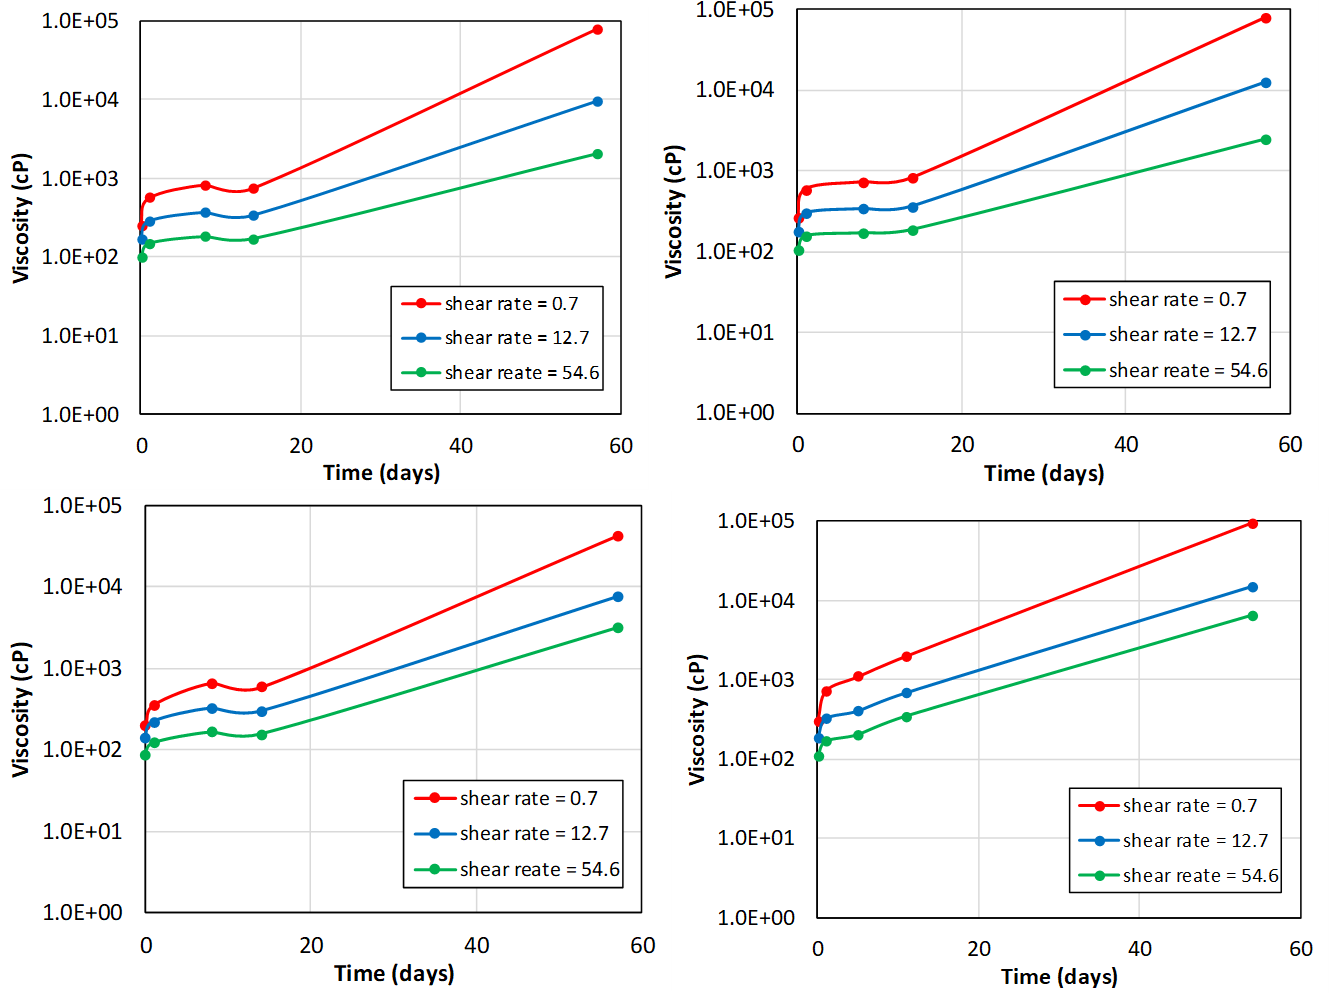
\includegraphics[width=1.2\textwidth]{img/cht/s17visc80.png}}
    \caption{Polymer/PEC solutions aged at 80~\celsius. Upper left: Series 17 samples. Upper right: Series 18 samples. Lower left: Series 19 samples. Lower right: Series 20 samples.}
    \label{cht:s17visc80}
\end{figure}

The figure shows that on the first day of aging, the viscosities in all solutions increased to some degree. Then all three solutions with PEC (Series 17 through 19) exhibited an almost constant viscosity for 14 days. After 57 days, a significant increases in viscosity was seen for all the three solutions. Due to summer holidays, there was no measurements taken between days 14 and 57, and it is not possible to know the exact length of the "constant viscosity period". After 14 days the samples in Series 17 through Series 19 were characterized as viscous fluids. The samples in Series 20 were prepared without PVS and thus without PEC. For this series, the solution was characterized as viscous fluid after 5 days and as week gel after 11 days. Comparison of the samples made with and without PEC shows that incorporation of the amine POSS in PEC reduced gel formation significantly. Surprisingly, no effect was observed by increasing the amount of PVS.

A solution made with Flopaam 5115 VHS and PEC (Series 38) is compared with the same polymer, gelled with \ce{Cr^{3+}} as cross binder (101 ppm, Series 1) in Figure \ref{cht:s38visc80}. The polymer concentration was 1.00 wt.\% and the concentrations of amine POSS and PVS were similar to those of Series 17. Series 38 was aged at 80~\celsius~whereas Series 1 was aged at 50~\celsius.

\begin{figure}[h]
    \centering
    \makebox[\textwidth][c]{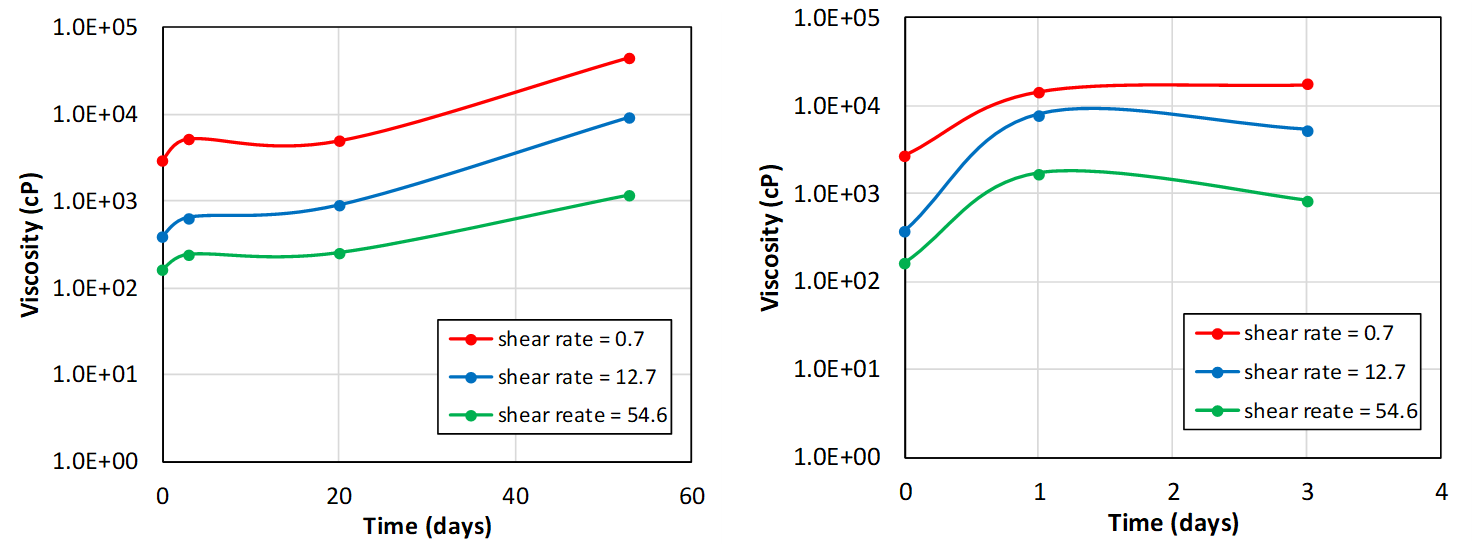
\includegraphics[width=1.2\textwidth]{img/cht/s38visc80.png}}
    \caption{Aging of samples in Series 38 made with Flopaam 5115 VHM/PEC and aged at 80~\celsius~(left), and of the same polymer with \ce{Cr^{3+}} (Series 1) and aged at 50~\celsius~(right).}
    \label{cht:s38visc80}
\end{figure}

By comparing Figures \ref{cht:s17visc80} and \ref{cht:s38visc80}, it can be seen that the viscosity in polymer/PEC systems made with Alcomer 24 UK as well as the ones made with Flopaam 5115 VHM showed an initial increase, and then plateaued before further increase. The period for constant viscosity lasted until at least 20 days, but could have been longer as there were no measurements between 20 and 53 days. The viscosity of Series 1 samples, aged at lower temperature, increased quickly as the result of gel formation.

Figure \ref{cht:s41visc80} compares polymer/PEC solutions where the concentration of Flopaam 5115 VHM was reduced to 0.50 wt.\% (Series 41). Series 41 was made with the same concentration of amide POSS (0.38 wt.\%) and of PVS (0.054 wt.\%) as Series 38. 

\begin{figure}
    \centering
    \makebox[\textwidth][c]{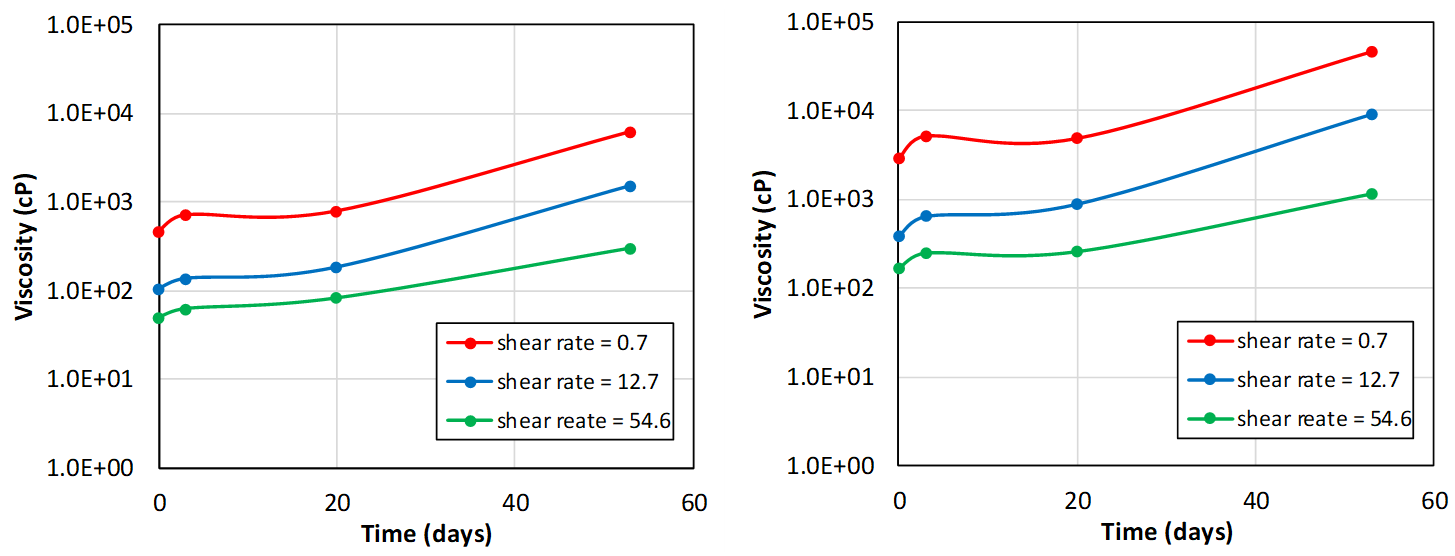
\includegraphics[width=1.2\textwidth]{img/cht/s41visc80.png}}
    \caption{Polymer/PEC solutions aged at 80~\celsius. Series 41 samples (left) and Series 38 samples (right).}
    \label{cht:s41visc80}
\end{figure}

The behavior of the Series 41 samples was comparable to that of Series 38 samples, however the measured viscosities were lower for Series 41 due to lower polymer concentration.

In Series 44, the concentrations of both amide POSS and PVS was reduced by a factor of two and the polymer concentration was kept unchanged compared to Series 17 (cf. Table \ref{tab:polyPecComp}). In Series 45, the concentrations of both amide POSS and PVS were reduced by a factor four compared to Series 17, still keeping the polymer concentration unchanged. Viscosities vs. time are compared in Figure \ref{cht:s44visc80}. The figure also shows the behaviour of the same polymer cross-linked with 104 ppm \ce{Cr^{3+}} (Series 3). Reduction of of PEC concentration reduced the rate of cross-linking. At the lowest concentration of PEC, cross-linking did not start at all in the aging period. As expected, the use of \ce{Cr^3+} as cross-linker resulted in fast gelation.

\begin{figure}
    \centering
    \makebox[\textwidth][c]{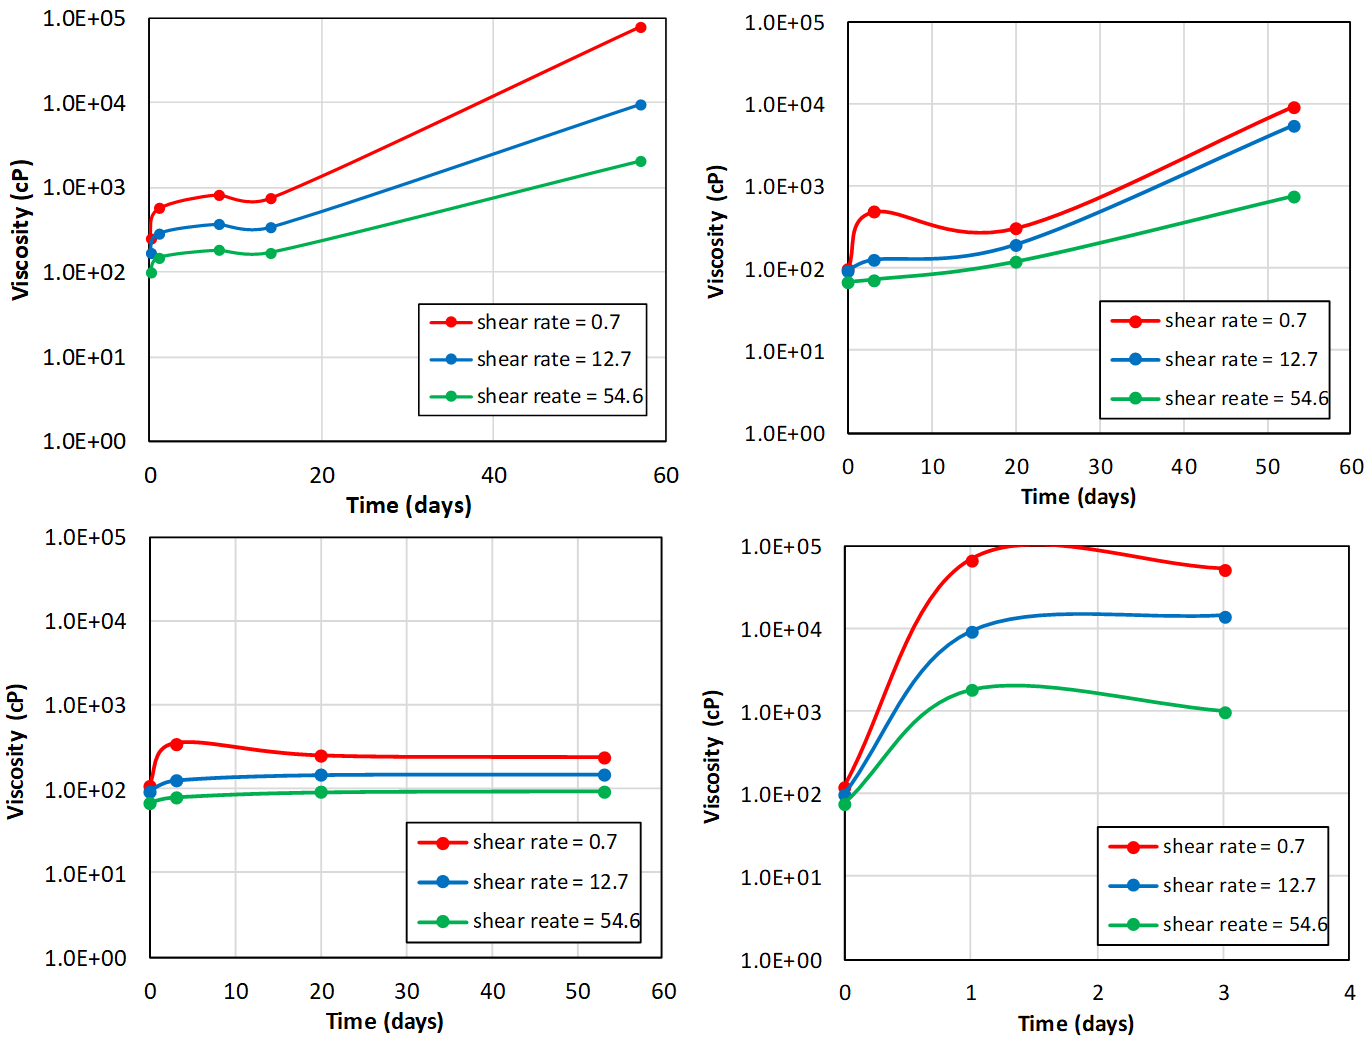
\includegraphics[width=\textwidth]{img/cht/s44visc80.png}}
    \caption{Aging of samples in Series 17 (upper left), Series 44 (upper right) and Series 45 (lower left) made with Alcomer 24 UK and aged at 80~\celsius, and of the same polymer with \ce{Cr^{3+}} (Series 3) and aged at 50~\celsius~(lower right).}
    \label{cht:s44visc80}
\end{figure}

\subsection{Gels based on lactamide POSS}
Figure \ref{cht:s23visc80} shows measured viscosities for the samples collected early and at the end of the injection during Experiment 1 (cf. Section \ref{sec:inSituGelling}). Except for the sample measured after 12 days at 0.7 s$^{-1}$, a clear trend is seen in the figure showing a slow increase in viscosity the first 25 days and then a faster increase thereon.

\begin{figure}
    \centering
    \makebox[\textwidth][c]{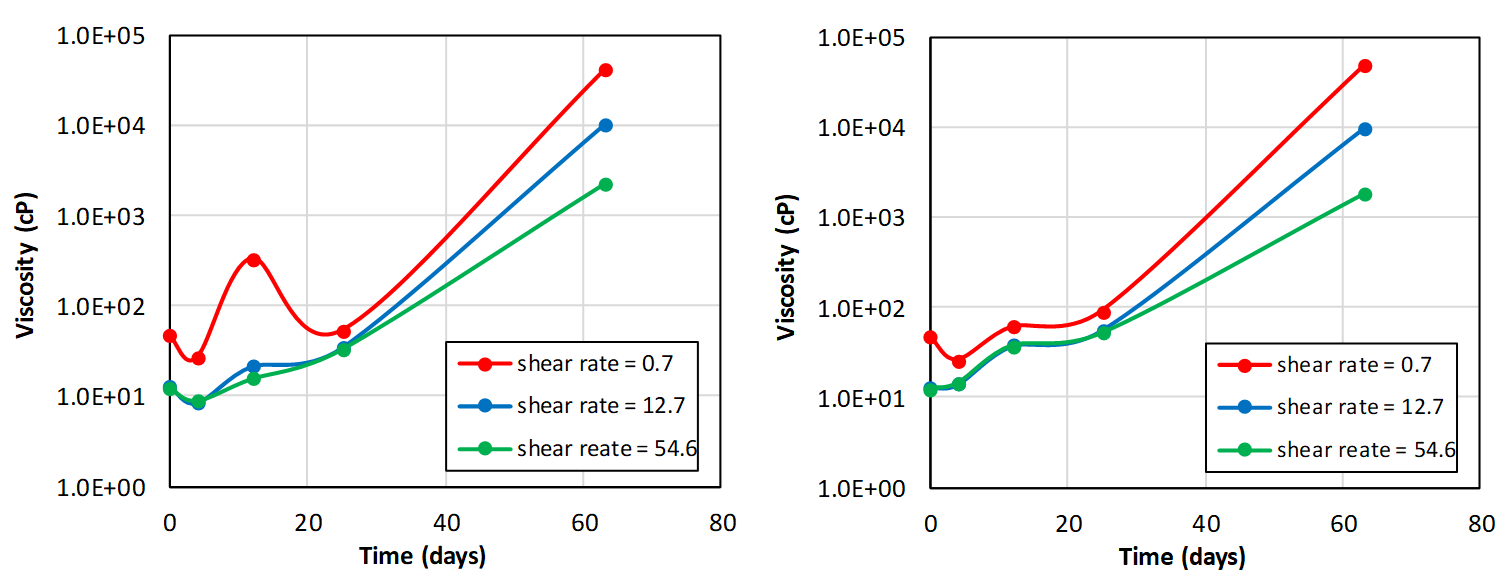
\includegraphics[width=\textwidth]{img/cht/s23visc80.png}}
    \caption{Aging of solutions in Series 23 collected during injection of nanoparticle/polymer solution in a core. Samples collected early (left) and collected at the end of the injection (right).}
    \label{cht:s23visc80}
\end{figure}

\section{Transport of polymer and nanoparticles through porous media}
\subsection{Injection of nanoparticles in Bentheimer sandstone}












\section{ Effect of in-situ gelling on water flow}